\begin{savequote}[9cm]
Begin at the beginning, the King said gravely, and go on till you come to the end: then stop.
\qauthor{--- Lewis Carroll, \textit{Alice in Wonderland}}
\end{savequote}


\chapter[Conclusion: How the Idea of Terrorism Is Changing Us]{Conclusion \\ How the Idea of Terrorism Is Changing Us}
\chaptermark{Conclusion}
\label{chap:chap6}


\lettrine[loversize=-0.2,lines=1]{H}{}ow does terrorism affect people's social and political attitudes? And, second, how can we explain differences in attitudinal reactions between individuals and across societies? This research started from the observation that existing knowledge on these questions falls short in at least three ways. First, much of the empirical research on how terrorism influences attitudes is conducted in Western, and primarily American, settings, raising important questions about the generalizibility of some of the commonly used theories in the field today. Second, a narrow focus on individual-level cognitions and emotions disregards the crucial role played by the context in which the relationship between terrorism and attitudes takes place. Third, despite a burgeoning literature on this topic, there is still little engagement with the conceptualization of 'terrorism' (at least within most part of the social- and political-psychological literature on which I predominantly drew). To address these gaps, throughout this dissertation, I gradually developed a model that cuts across disciplinary boundaries to describe and explain how `terrorism' influences attitudes. I will now add the final building blocks to this model by taking a step back from the empirical findings and collectively consider them within the context of current debates on ``the power of terrorism'' \citep{Diplomat2016}. 


In what follows, I first substantiate how the empirical findings of this dissertation brought me to one overall, theory-building conclusion (Section \ref{sec:61}). By doing so, I provide answers---albeit preliminary ones---on the two overarching research questions that have guided this dissertation and show how this dissertation contributes to both academia and the society-at-large. Then, I look inward by, first, reflecting on how my own positionality has impacted this research project and its outcomes (Section \ref{sec:622}) and, second, discussing the thesis' main limitations (Section \ref{sec:621}). Next, I propose avenues for future research inspired by the results and remaining questions of this doctoral project (Section \ref{sec:63}). Finally, I conclude on a more personal note with one final thought (Section \ref{sec:64}).



%By emphasizing and explaining the differences between terrorism and the \textit{idea} of terrorism, this dissertation makes four major contributions to the existing literature: an empirical, conceptual, theoretical, and societal one. First, it highlights that this \textit{idea} of terrorism is context-depending but that we, at the same time, know surprisingly little about how different societies construct the \textit{idea} of terrorism. By combining a cross-national approach with an in-depth study of a non-Western case, this dissertation took a vital step in addressing this academic gap. Second, it demonstrates that the particular way in which people in a given society talk about terrorism is part of the answer of how this \textit{idea} is affecting their socio-political attitudes. By starting to document how people in non-Western societies talk about `terrorism,' this dissertation allows a more critical engagement with this concept. Third, both of these observations underline the importance of taking a country's socio-demography, and particular its intergroup relations hierarchy, into account---adding an important theoretical nuance to the existing literature. By means of the empirical, conceptual, and theoretical contribution, findings from this dissertation equally contribute to the society-at-large. Indeed, we can only start looking for solutions once we properly understand the problem at hand. Once we understand when, why, and how citizens react to particular forms of violence, we can start thinking about proper guidelines, strategies, and interventions to counter potential democratic backlashes and build more resilient citizens and societies. Offering such guidelines based on rigorous academic insights was the ultimate goal of this dissertation.



\section{Looking Backward: Conclusions and Contributions}
\label{sec:61}

In essence, this dissertation set out to gain a deeper understanding of the implications of `terrorism' for people's social and political attitudes in both Western and non-Western societies. To do so, throughout the empirical chapters, I took stock of specific terrorism-induced attitudinal changes, examined mediators explaining the relationship between terrorism and attitudes, and assessed various moderators strengthening or weakening this relationship. Each of the chapters provided some interesting insights in this regard. In Chapter 2, we started off by discovering how \textit{terrorism} and \textit{terror} are two separate constructs, in which the latter is particularly damaging for generalized trust within more democratic and less terrorist-prone countries. Television news consumption was also found to extend the reach and effects of the terror of terrorism. In Chapter 3, we learned how Nigerian young adults, regardless of their religious background or terrorism exposure, are driven by signs of repentance, reconciliation, and remorse when making judgments about post-conflict reintegration, and that respondents' belief in the success of reintegration seems to be an important mechanism driving these effects. We also found out, through the content analysis in Chapter 4, that both a Muslim- and Christian-affiliated newspaper in Nigeria did not repeatedly attribute the root cause of Boko Haram's violence to Islam and Muslims as such, and that both papers reported on the violence in very similar ways. Last, the meta-analysis in Chapter 5 illustrated that much of what we know about how the public reacts to terrorism is based on violence perpetrated by Islamist actors within Western countries. At the same time, the empirical evidence suggested that responses to political violence committed by other actors may be much weaker (or even non-existent). Now, how can we collectively make sense of these separate empirical findings?



\subsection{Overarching Conclusion}
\label{sec:611}
In this overarching conclusion, I substantiate how the empirical findings jointly contribute to the following three-fold conclusion: 

\begin{enumerate}[noitemsep]
    \item Not terrorism as such, but rather the \textit{idea} of terrorism is changing us. 
    \item This idea relates to the question ``\textit{what/who} do we talk about when we talk about terrorism?''
    \item What/who we talk about when we talk about terrorism is to a large extent determined by \textit{specificities of the intergroup context} in which violence takes place.
\end{enumerate}

\subsubsection{Proposition 1: The \textit{Idea} of Terrorism is Changing Us}

In 1929, Thomas and Thomas published what is often considered one of most important sentences in the Social Sciences---that is, ``[only] if men define situations as real, they are real in their consequences'' (p. 572; as cited in Stampnitzky, \citeyear{Stampnitzky2013}, p. 5). Several chapters in this dissertation equally suggest that for `terrorism' to have real consequences for citizens' social and political attitudes, it first needs to be perceived as such. So, how we think and talk about `terrorism'---or, in other words, how we construct the \textit{idea} of terrorism---might be a crucial part of the answer of how this construct is changing us. For example, concerns over the likelihood of another terrorist attack---a strong predictor in much previous work \citep[e.g.,][]{Huddy2005, Davis2004, Cohrs2005a}---was not significantly related to generalized trust in less democratic and more `terrorist'-prone countries (Chapter 2). Also, neither terrorism exposure nor anger appraisals did moderate the results of our conjoint experiment conducted among university students in Nigeria (Chapter 3), whereas these factors turned out to be particularly strong predictors of public responses to terrorism in Western countries (Chapter 5; see also Vasilopolous et al. \citeyear{Vasilopoulos2018, Vasilopoulos2019c}; Marcus et al. \citeyear{Marcus2019}). This suggests that people in different countries might define and perceive contentious and violent situations in starkly different ways.

%How can we adapt our theoretical lenses to equally account for these puzzling results? 

Therefore, I argue that answering the central questions of this dissertation requires examining the differential labeling and intersubjective understanding of violent acts by several actors.\footnote{I derived the phrase “intersubjective understanding” from Alexander Wendt (\citeyear{Wendt1992}). It denotes that all meanings ``arise out of interaction'' (p. 403).} People might perceive similar acts of political violence in different ways because the way in which we understand particular acts of violence depends to a large extent on our interactions with relevant others (including fellow citizens, politicians, and media messages). Such social interactions, or intersubjectivity \citep{Duranti2010}, form the basis of the dominant assumptions of who is more likely to be a `terrorist' within a given political-geographical context at a given moment in time. Yet, who is more likely to be a `terrorist,' and hence to elicit sociopolitical reactions, within a given society---and why?



\subsubsection{Proposition 2: The Idea of Terrorism is Based on \textit{What/Who} We Talk About When We Talk About Terrorism}

To break down this second proposition, let me begin by asking the following question: If terrorism is defined as the tactic of using, or threatening to use, violence to generate a psychological effect in order to achieve a political goal (see academic consensus definition in the introduction), then how do we account for the fact that certain groups and ideologies are more likely to be called 'terrorist' compared to others perpetrating similar acts within the same cultural and political sphere? The tendency of today's Western politicians, journalists, and citizens to call violence perpetrated by Muslims `terrorist,' as opposed to violence by white perpetrators, is well-documented \citep{Kearns2019, Powell2011}. Additionally, even when similar acts by various kinds of perpetrators are labeled `terrorism,' white supremacists violence still receives less attention and leads to weaker political and legal consequences compared to Islamist violence \citep{Malik2020, Meier2019}. This dissertation adds to this debate in at least two ways.


First, it shows that citizens' attitudinal responses in the wake of `terrorism' also depend to a large extent on the identity of the alleged perpetrators. More specifically, in the West, violence allegedly perpetrated in the name of the Islam leads to a stronger increase in political conservatism and out-group hostility. In contrast, violence \textit{not} associated with the Islam leads to weaker or insignificant attitudinal reactions (Chapter 5). Second, we also discovered that---besides politicians, journalists, and citizens---scholars are equally vulnerable to the broader discourses that make violence in the name of certain ideologies more `thinkable' as terrorism. More specifically, more than half of the existing empirical studies on terrorism and political attitudes pertain to Islamist terrorism, whereas not even 5 percent investigates the attitudinal implications of extreme right-wing terrorism (Chapter 5). This finding is in line with Moore's (2015, p. 356) observation that:


\begin{quote}
    ``... the concepts we [i.e., scholars] use in our theories are not immune from the political usage of words in daily politics. ... we tend to be trapped by the implicit cultural and political assumptions of our time.'' 
\end{quote}
\newpage

It is important to note in this respect that the vast majority of previous work on---and thus our theoretical knowledge about---public reactions to terrorism draws on insights derived from the United States, Israel, and Europe and the repercussions of the 9/11 attacks, the intractable Israeli-Palestinian conflict, and a several ISIS attacks. While this literature has provided valuable insights, this dissertation demonstrates how generalisations beyond these particular contexts remain, at best, complicated. In particular, Chapter 5 showed that, across the Western-dominated literature, `they' primarily refers to Muslims hurting 'us, Westerners,' whereas this post-9/11 'us-versus-them' narrative was not so straightforward for the Nigerian journalists interviewed or in their news messages scrutinized in Chapter 4. Therefore, the last part of the overarching conclusion adds that, besides ``cultural and political assumptions of our time'' (Moore, 2015, p. 356), it is of equal importance to take the assumptions of the specific context, and particularly the \textit{intergroup context}, into account.


\subsubsection{Proposition 3: The Terrorism/Terrorist Idea is \textit{Intergroup Context}-Dependent}
As explained before, people are inclined to divide the world into in- and out-groups and to derive a ``positive social identity'' from favorable comparisons between the in-group and relevant out-groups. Because of the pervasiveness of such social categorization and comparison processes, ``in-group bias is a remarkably omnipresent feature of intergroup relations'' \citep[p.~38-40; see also Brewer, \citeyear{Brewer1981}; Hewstone, Rubin, \& Willis, \citeyear{Hewstone2002}]{Tajfel1979}. Building on these notions, terrorism then becomes violence `they` (i.e., a prominent out-group) inflict on `us' (i.e., the in-group) and, as a result, `we' will react socially and politically stronger when the alleged perpetrator of violence is one of `them.' Importantly, while such social categorization processes cut across national boundaries and cultures, a particular social identity will always be embedded within a given social and political context \citep{Hewstone2002}. More specifically, this dissertation suggests that the concrete interpretation of `them' and `us' might depend on \textit{specificities of the intergroup context} in which people are embedded and in which violence takes place. This final remark is crucial to comprehensively understand how terrorism influences people's social and political attitudes across societies. Attitudinal responses to `terrorism' might differ across societies because all people tend to divide the world into in- and out-groups, but the specific \textit{boundaries} (i.e., conflict fault lines) and \textit{dynamics} (i.e., numerical ratio and power hierarchies) between those groups often differ across societies.\footnote{And time periods. Yet, a historical assessment of this argument is outside the scope of this thesis.}
\newpage

As Chapter 2 demonstrated, concerns over the likelihood of terrorist attacks decreased social trust most strongly in more democratic countries. The above-mentioned and final argument of this dissertation equally helps to further explain this finding. That is, trust might be more affected in more democratic countries because the majority of terrorist attacks\footnote{Or, at least, those incidents labelled and counted as ‘terrorist’ by the Global Terrorism Database and, hence, included in our model.} in those countries—--which are predominantly situated on the Western hemisphere of the world (e.g., the U.S., Germany, the Netherlands, Spain)—--are perpetrated by a clearly defined, often fairly small, and relatively marginalized out-group. By contrast, terrorist attacks in the included less democratic countries (e.g., Bahrain, Yemen, Russia, Iraq) often take place in less clearly delineated and starkly different intergroup contexts. In this regard, I propose that both intergroup boundaries and dynamics may significantly shape public responses to terrorism. 


First, sociopolitical reactions---and in particular feelings of out-group hostility---especially occur when terrorists have clear and exclusive ties with a particular out-group.\footnote{Interestingly, recent research on the strategies of terrorism also suggests that insurgents might use terrorist tactics strategically to exacerbate intergroup boundaries \citep[][p. 2031]{Polo2020}.} As Chapter 5 demonstrated, majority citizens in Western countries were found to react politically and socially stronger when the violence was committed by an Islamist, and thus out-group, organization or individual. In contrast, their reactions to far-right or state terrorism---where intergroup distinctions are less clear---were significantly weaker. Second, once the fault lines within a conflict are clear, demographic realities and group-based power hierarchies further shape public responses to terrorism. In this regard, Chapter 4 outlined how the status of religious groups may influence media reports of religious-based violence. Building on intergroup contact theory \citep{Pettigrew2006, Pettigrew2008a}, we argued that more frequent inter-religious contact between citizens in general and within the newsroom in particular, as well as more equal divisions of political power, might encourage journalists to cover religious-based violence in a more balanced way.\footnote{In addition, intergroup boundaries are also less distinct in Nigeria given that Boko Haram is also as seen an insurgency against the state and its economic realities (see also Appendix \ref{app:A2}). I would like to thank the anonymous reviewer of my dissertation for this important addition.} Now, I propose that such micro- and macro-level features of the intergroup context may also have a more general impact on how political violence is perceived and responded to by citizens (as well as studied by scholars). Both a country’s demography and political power distributions may shape the status of in- and out-groups and, thereby, prompt a political process in which the terrorist label will be preserved to categorize a particular out-group.


Specifically, the larger and politically more powerful an in-group, the more likely it becomes that such out-group categorization process will occur. Antonio Gramsci’s concept of cultural hegemony further formalizes this idea by illustrating how a ruling `in-group' may exert power in a society such that the group's ``values, norms, perceptions, beliefs, sentiments, and prejudices'' become the legitimate dominant ideology \citep[][p.569]{Lears1985}. Following institutional scholarship, political and societal elites might thus create sticky ``rules of the game,'' advantaging some groups over others and presenting that intergroup hierarchy as natural and inevitable (North 1990). As a result, violence perpetrated by particular groups `lower' in the hierarchy and challenging the inevitability of this hierarchy constitutes an exceptional existential threat or, hence, `terrorism.'  Terrorism---as well as counter-terrorism policies, for that matter \citep[][]{Meier2019, Fadil2019}---thus becomes a tool often deliberately and strategically utilised by politicians to uphold the status quo. As this dissertation has shown, this political tool equally causes citizens to react more strongly to violence committed by out-groups and, thus, more often framed as `terrorism.' 


Anno 2020, these intergroup hierarchies might not just be society- or state-specific, but also play out at a regional and perhaps even global level. As Chapter 5 illustrated and several scholars noted before \citep{Meier2019, Fadil2019, Holland2012}, 9/11 became a fulcrum for global understandings of terrorism and colored policies, discourses, and scholarship on terrorism internationally. Muslim populations in particular became the prime target of counter-terrorism policies \citep[see, e.g.,][]{Kundnani2014}, terrorism discourses \citep[see, e.g.,][]{Kearns2019, Powell2011}, and terrorism scholarship (see Chapter 5)---especially within the West. On the other hand, the Nigerian chapters suggested that, first, when the fault lines within a conflict become more versatile and less distinct and, second, when groups within a society become more similar in size and power, this classification process may take a different form. Importantly, while the Nigerian studies provided crucial first insights into these processes, the full extent of the implications of intergroup relations on the construction of the idea of terrorism, particularly in non-Western contexts, remains under-explored (see also avenues for future research in Section \ref{sec:63}).

\newpage

\subsubsection{Putting the Pieces Back Together}
In short, this dissertation concludes that people---including citizens, politicians, journalists, ànd academics---tend to construct the \textit{idea} of terrorism, at least in part, based on \textit{specificities of the intergroup context} within a given society at a given moment in time. This idea, in turn, influences our social and political attitudes. More specifically, sociopolitical reactions are thought to especially occur among a dominant in-group when terrorists have clear ties with a disadvantaged out-group. As a result, centering the ``cultural and political assumptions of our time'' and society within the academic study of terrorism, and noting that they are temporally and geographically fluid, is crucial to understanding how ‘terrorism’ is changing us. 

This overarching conclusion brings us back to the `idea of terrorism' introduced in the conceptual and theoretical framework of this dissertation. I've come full circle by proposing that this idea, including the practices and discourses of terrorism and counter-terrorism, is to a large extent based on the intergroup boundaries and dynamics---including the demarcation of in- and out-groups, frequency of intergroup contact, and distribution of power---within a certain society at a particular moment in time. Figure \ref{fig:conclusion} visualizes this theory-building conclusion in which the intergroup context is hypothesized to be an important scope condition enabling a chain of reactions to certain acts or threats of violence---or not.


%----------------------------------------------------------
% Figure 1: Conclusion
%----------------------------------------------------------
\vspace{3mm}
\begin{figure}[H]
\fbox{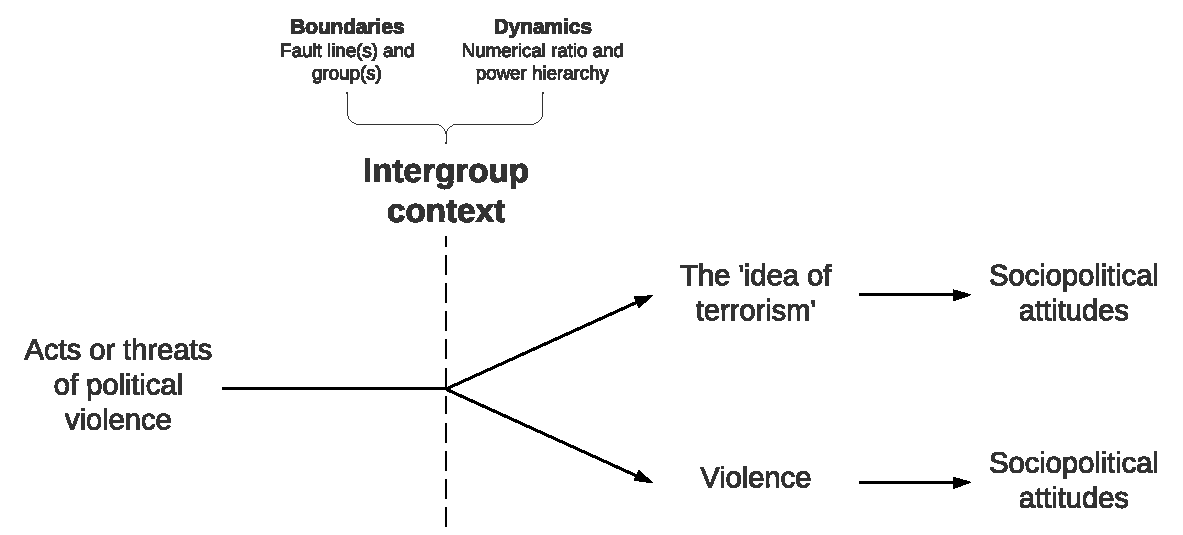
\includegraphics[width=\textwidth]{Chapter_6/conclusion-figure1.pdf}}
\caption{How the Intergroup Context Shapes the Relationship between Acts or Threats of Political Violence and Sociopolitical Attitudes}
\label{fig:conclusion}    
\end{figure}
%----------------------------------------------------------



%While this dissertation studied how this `idea of terrorism' impacts attitudes, it is important to end this conclusion by putting it in perspective. `Terrorism,' first and foremost, destroys human lives. About 3,000 people lost their lives on that blue-sky Tuesday morning in September, 2001. Since May 2011, an estimated 38,655 people---including civilians, state actors, and Boko Haram members---have been killed in the Boko Haram conflict and roughly 2,5 have million people fled their homes.\footnote{Estimate retrieved via \href{https://www.cfr.org/nigeria/nigeria-security-tracker/p29483}{the Council on Foreign Relations' Nigeria Security Tracker} on May 27, 2020.} Yet, the {idea} of terrorism equally destroys human lives. About half a million people in Iraq, Afghanistan, and Pakistan lost their lives in the post-9/11 Global War on Terror \citep{Crawford2018}.\footnote{That many of `us, Westerners' tend to be oblivious to these relative numbers can also be related to the intergroup power dynamics central to this dissertation.} The idea of terrorism also damages a country's economy \citep{Enders2016, Enders2012} and affects its polity and the rule of law \citep{Bigo2015, Kundnani2014, Wilkinson1986}. So, at a time characterized by continuous disagreements on how to define 'terrorism' \citep{Richards2019}, the {`idea} of terrorism' seems to have a pervasive impact in many different ways on many different societies.



%This idea became clear in Chapter 4, where we saw that, because the socio-demographic reality in Nigeria, the \textit{idea} of terrorism was constructed quite different compared to western constructions of `terrorism. These differences in reporting might also explain some of the null results found in Chapter 3. 

%Such reasoning is also in line with some anecdotal evidence. Over the course of this dissertation, I repeatedly noticed the tendency of the Flemish national television to broadcast a new report about, for example, a terrorist attack causing 200 deaths in Pakistan right before the sports and after a series of Flemish trivia, while far less lethal attacks in Western countries were often worth opening the news with. These tendencies are, at least in part, an expression of our deeply ingrained social identity.\footnote{Even though classic new values theory does not use this intergroup relations language, they \dots}

%terrorism is not an abstract conception of violence but always anchored in a specific social and political context.

\newpage
\subsection{Main Contributions and Implications}
\label{sec:612}
In this section, I highlight the empirical and methodological as well as theoretical and conceptual contributions of this dissertation, and explore consequent implications for how we understand and study `terrorism.' These scientific contributions, in turn, provide potentially useful insights for the society-at-large because, once we understand when, why, and how citizens react to particular forms of violence, we can start thinking about guidelines, strategies, and interventions to build more resilient citizens and societies in times of `terror.'

\subsubsection{Empirical and Methodological Contributions}
This dissertation has made several empirical and methodological contributions to the literature on public reactions to terrorism. First and foremost, I have argued and demonstrated how insightful research in non-Western contexts might be for the study of terrorism. Boko Haram constitutes an organization designated `terrorist' by national governments \cite[e.g.,][]{Canada2013, USState2020}, the United Nations \citep{UNSC2014}, think thanks \citep[e.g.,][p. 4]{InstituteforEconomics&Peace2015}, and academics \citep[e.g.,][]{Aghedo2012, Godefroidt2018a} alike. Yet, I could not retrieve a single study (besides my own) quantifying the relationship between exposure to Boko Haram violence and any form of political or social attitudes. Studies on Boko Haram predominantly focus on different aspects, such as the origins of and solutions for the conflict \citep[e.g.,][]{Onuoha2010, Iyekekpolo2016a, Mustapha2014b, Aghedo2013}, and those few studies analyzing how it has affected interfaith relations use qualitative methods \citep[e.g.,][]{Onapajo2015}. Notwithstanding the valuable insights these studies offer, the systematic study of how about 2,000 young Nigerians cope with Boko Haram violence and how about 700 news reports have talked about this violence constitutes, in my opinion, a crucial empirical contribution. As we have seen, this empirical data not only provided extremely timely information for Nigerian authorities, it also offered highly instructive theory-building insights. 


Second, this dissertation has drawn on multi-level structural equation models (Chapter 2), a conjoint experiment (Chapter 3), a mixed-methods design combining in-depth interviews with a quantitative content analysis (Chapter 4), and a three-level meta-analysis (Chapter 5) to advance knowledge on how terrorism is changing us. By doing so, this dissertation has demonstrated how various innovative research designs can be combined to gain both deeper and broader insights into the effects of terrorism, and illustrated the importance of expanding our methodological scope beyond single case-studies. Moreover, I tried to apply these methods as rigorous and transparent as possible. Over the course of my doctoral journey, I became increasingly aware of and involved in the Open Science community. Honestly, this was---and still is---a learning process. Yet, nowadays, I share my data and analysis code whenever possible (as has been done in all but the first chapter of this dissertation) and all my later work, including the meta-analysis in this dissertation, has been preregistered (especially when conducting confirmatory research). I hope this work can encourage others in the field of terrorism effect studies to equally engage with Open Science practices---especially regarding preregistration given that only ten studies in my meta-analysis were reported as preregistered.


\subsubsection{Theoretical and Conceptual Contributions}
Next, this dissertation has implications for our theoretical perspective on terrorism and its attitudinal effects by emphasizing, first, the importance of interdisciplinary integration in general and, second, the need to pay closer attention to the intergroup context in particular. Concretely, the framework outlined in Chapter 1 incorporated theoretical insights originating from political sciences and media studies into the fields of social and political psychology. While all elements in this framework thus stem from existing theories, the contribution here was to put these pieces together and highlight important parallels between distinct disciplines. Furthermore, this framework was grounded in a comprehensive conceptualization of `terrorism' by looking at both practices and discourses of acts and threats of violence by various actors. Altogether, throughout the dissertation, both micro-level and macro-level factors were taken into account and `terrorism' was comprehensively, and increasingly critically, measured and studied. 


As a result of this interdisciplinary and critical approach, the main theoretical contribution of this dissertation has been to introduce the intergroup context, and particularly intergroup contact and power hierarchies, within the field of terrorism effects studies. As we saw in the previous Section (\ref{sec:611}), this intergroup perspective is important to get a better understanding of both the effects of terrorism on attitudes as well as of the concept of terrorism as such. Despite the vast literature on how the public responds to terrorism \citep[e.g.,][]{Gadarian2010c, Davis2004, Vasilopoulos2019c, Larsen2020} and a wide range of academic and policy definitions of terrorism \citep{Richards2014, Schmid2011, US2019}, the majority of these studies and definitions have failed to explicitly acknowledge the intergroup dynamics underlying this concept and to address subsequent assumptions underscoring any study on `terrorism.' This is remarkable given the prominence of intergroup relations within the fields of social and political psychology. In addition, putting intergroup relations center stage in the study of terrorism holds the potential to generate testable hypotheses about which acts of violence are more likely to be perceived as `terrorism' within a given society at a particular moment in time and, hence, which acts are more likely to `terrify' and elicit a sociopolitical response. As Chapter 5 has demonstrated, Islamist terrorism seems to elicit a particularly strong attitudinal response within the West these days, yet the Nigerian chapters have suggested that the full extent of the repercussions of Islamist terrorism in non-Western contexts remains under-explored. 


\subsubsection{Societal and Normative Implications and Recommendations}
The proposition that not terrorism as such, but rather the idea of terrorism, is changing us holds important implications for how we---citizens, journalists, politicians, and academics alike---apply and respond to the term `terrorism.' In addition to the broader implications of this overall conclusion, each individual chapter also entailed specific implications for those four stakeholders. In what follows, I shortly outline how both this dissertation and its empirical chapters entail certain normative implications and recommendations for citizens, journalists, politicians and academics.


First, regarding citizens, an important finding of this dissertation is that people are more reactive to out-group and indifferent to in-group threats, and that emotions play a crucial role in this process. Building more resilient citizens and cohesive societies might thus entail raising awareness of such biases and emotional responses. Recently, Pliskin and Halperin (\citeyear[][p. 93]{Pliskin2020}) similarly noted that ``tolerant societies are societies that individually and collectively cope better with negative intergroup emotions.'' They, therefore, advocate for the use of so-called cognitive reappraisal interventions---a strategy that entails contemplating on a situation's meaning in a way that positively affects its emotional impact \citep[for more information, see][]{Pliskin2020, Halperin2014}. In line with this, this dissertation suggests that, in many of today's Western societies, it might be of particular importance to learn how to cope with the emotions of fear and anger in the wake of out-group violence. Especially pointing out, first, the relative danger of terrorism to alleviate concerns over future attacks (based on Chapter 2) and, second, our biased reactions in general and angry responses in particular to Islamist terrorism (based on Chapter 5) might offer promising strategies for many Western democracies. Regarding these biased reactions, Bruneau and colleagues (\citeyear{Bruneau2019}) recently demonstrated that ``an intervention that highlights the hypocrisy involved in collectively blaming out-group but not in-group members for the blameworthy actions of individual group members effectively reduces collective blame of Muslims and support for anti-Muslim policies'' (p. 45; see also Bruneau et al., \citeyear{Bruneau2018}).


Second, this dissertation calls upon journalists to be more cautious and less biased when using certain labels and frames. In this respect, Chapter 4 highlights how newsroom diversification might contribute to news differentiation. In other words, increasing the diversity within the newsroom might lead to a more careful coverage of religious-based violence in which violence is not attributed to a particular religion as such, but to a few extremists not representative for that religion. Importantly, emphasizing the responsibility of individuals instead of collectively blaming the out-group has indeed shown to attenuate out-group hostility in reaction to terrorism news reports \citep[][this is also in keeping with Bruneau et al.'s, 2020, `collective blame hypocrisy' intervention]{VonSikorski2017}. Of course, the recommendation to pay special attention to newsroom diversification and news differentiation assumes that journalists are largely unaware of and/or concerned about their biased reporting, and will probably not hold for those news organizations that deliberately apply `terrorism' labels and frames to pursue or support a certain agenda.


Third, this dissertation holds important implications for how political elites interact with their citizens in the wake of a terrorist attack. On the one hand, political leaders might exploit certain labels and frames to capitalize on the emotional and political reactions of their citizens in order to pursue a particular political agenda. For example, by labelling an out-group as `terrorist,' highlighting perpetrators' group identification, and/or stressing the differences between that out-group and the own in-group, politicians might be able to not only generate support for certain intrusive counter-terrorism policies but also further strengthen group boundaries. On the other hand, results from this dissertation might equally inspire leaders to interact with their citizens in such a way that it attenuates the emotional, social, and political repercussions of terrorism. In this regard, Chapter \ref{chap:chap3} outlined a specific roadmap for Nigerian politicians to effectively and efficiently communicate about the reintegration of ex-Boko Haram fighters.


Last, Chapter 5 has demonstrated how scholarly work on reactions to terrorism also reflects Western- and 9/11-centered ideas about `the enemy.' In other words, in addition to citizens, journalists, and politicians, scholars equally tend to follow a particular understanding of terrorism based on their own positionality and, thereby, play an important role in the construction of the `idea of terrorism' as well. It turns out that even in countries where far-right, racist, and/or antisemitic violence (or, indeed, terrorism) takes place, Islamist terrorism is still more likely to be studied. This dissertation, therefore, aspires to some critical reflection on the power of research in shaping the conversation about terrorism and, ultimately, calls for an increasing awareness of and transparency about the consequences of scholars' positionality within this body of scholarship (as I will also do regarding my own positionality in the next Section). In addition to affecting which particular acts or threats of violence have been investigated, such positionality has also resulted in a more generally Western-dominated field of study. The Nigerian chapters indicate that this might have obscured a deeper engagement with the full extent of the `enemy' construction. Indeed, the construction of the idea of terrorism within non-Western societies, and the role of different constellations of the intergroup context therein, remains poorly understood because our empirical and theoretical lenses are kept focused on the West. By studying such constructions within Nigeria, this dissertation contributes to and calls for further decentering current academic debates on `terrorism.' 


In short, the main societal implication of this dissertation can be summarized as follows: Words matter. Although responding strongly to out-group threats might be seen as functional from an evolutionary perspective \citep{Tooby2010, Lindner2018}, the fact that we do this reinforces the same biases that has lead us to respond in such strong emotional and political way in the first place. By systematically reacting differently to similar acts of political violence by different actors, we maintain the very same categorization processes and power hierarchies that underlie our reactions. Therefore, many stakeholders within society might need to be more careful when using and responding to certain words or, conversely, react with equal vigilance and strength to in-group violence. Should we then simply abandon the term `terrorism' altogether? No, in my opinion. First, it is probably an illusion to believe that the term will disappear from popular discourses because scholars decided this is the best thing to do. As explained above, the terrorism discourse can be very useful for certain actors pushing a particular agenda. Second, regarding scholarly usage of the term, it is important to note that conceptual disagreement is not unique to the field of terrorism studies (see, e.g., current debates on `populism'). Last, although this dissertation demonstrates how scholars (at least within the field of terrorism effects studies) might be prone to the same subjective errors as the general public, I would not recommend erasing `terrorism' from our dictionary right away. Instead, I would like to suggest that defining and studying `terrorism' entails deducing \textit{which identities and corresponding power structures} are perceived as under threat by \textit{which actors}.


\newpage
\section{Looking Inward: Positionality and Limitations}
\label{sec:62}


\subsection{Positionality}
\label{sec:622}
A first important aspect of `looking inward' is to reflect on how my positionality as a young, European, left-leaning, and female scholar has influenced this research project and its outcomes. For a long time, I actually believed that I minimized or even eliminated such influences by primarily conducting quantitative research.\footnote{An assumption that is also reflected in the fact that, while writing this section, I mainly found sources on how to use a reflective approach in relation to \textit{qualitative} research.} But, as Moors (\citeyear{Moors2019}) aptly points out, a completely neutral and unbiased researcher is like an ``imaginary tabula rasa'' and it is, therefore, crucial to ``reflect on our own positionality and develop an awareness of the assumptions we [i.e., researchers] all work with'' (p. 253). 


To begin with, the questions central to this dissertation reflect my social and political worldviews. This is evident, for example, in the introductory anecdote or the concluding quotes. More generally, I deliberately choose to advance knowledge on a particular social phenomenon in order to generate a \textit{desired} change and counter an \textit{undesired} response. As a result, I was---and still am---emotionally involved with the topic and subjects I studied. It is important to emphasize here that contributing to society motivates many scientists and that I consider this, as well as emotional involvement, an added value rather than a potential source of bias. Second, my positionality also affected the secondary sources and theoretical perspectives I have relied on. I became especially aware of my Western-centric understanding of this topic when some of the theoretical frameworks I tested did not replicate within the Nigerian context or when some of our survey questions were interpreted differently than intended by our pilot respondents or my Nigerian colleagues. Given my background, it is almost inevitable that I still missed particular nuances of the Nigerian context and that some of my participants might feel that my conclusions do not properly reflect their opinions and experiences. Not only my geographical background, but also my gender influenced the sources I used. For over a year now, I turn my writings through the Gender Balance Assessment Tool (\href{https://jlsumner.shinyapps.io/syllabustool/}{GBAT}; Sumner, \citeyear{Sumner2018}) and pay particular attention to use sources authored by female scholars as women remain underrepresented in scholarly work.\footnote{For your information, approximately 33.73 percent of the authors of the secondary sources used in this dissertation are women.} Third, as one might have noted, this dissertation departed from a positivist stance (in Chapter 2 and 3) to study discourses (in Chapter 4) and knowledge production (in Chapter 5) on `terrorism.' This critical turn was primarily data-driven and grounded in existing social and political-psychological theories. Additionally, it is in line with a more general trend in the field of terrorism studies whereby the discipline is evolving into a more critical and normative discipline that questions the dominant realistic and positivist problem-solving tradition \citep{AlKassimi2019}. I cannot, however, fully exclude the possibility that this critical turn was partly caused my worldviews as well. Last but definitely not least, my background had a crucial impact on my exploratory fieldwork in Nigeria. During this fieldwork, I became increasingly aware of my \textit{self}---being a young, European, non-Muslim woman in Nigeria. This `outsider' position entailed both advantages and disadvantages: My European background sometimes facilitated access to high officials, whereas my religion and gender impeded some in-depth interviews with religious leaders. For example, I will never forget how a Christian leader was reluctant to continue an interview because I was unable to list all ten commandments or how Muslim leaders often requested the presence of a male Muslim and refused to look me in the eye during our conversation. And while I conducted my interviews and focus group discussions in English without a hitch, I noticed at times that I had problems understanding some of the accents or that some participants returned to so-called Pidgin English. Therefore, both a local Nigerian and I transcribed (most) interviews and focus group discussions.


In sum, my positionality shaped several of my research activities---from formulating my research questions and hypotheses to collecting and interpreting my data. I believe that the above reflection does not undermine my research results,\footnote{Therefore, I also separated this section from the next Section on limitations (Section \ref{sec:621}).} but rather adds additional insights into the complex and multi-layered dynamics underlying each research project. Furthermore, not only did I impacted this research project by bringing in my own assumptions and backgrounds, this project also impacted me as a person.\footnote{Reflecting on ``the effects of the research on the researcher'' is sometimes called \textit{retrospective} reflexitivty and complements the \textit{prospective} reflexivity outlined above \citep{Attia2017}.} For example, today, I am much more aware of intergroup biases present in many (Flemish) news reports or in many of the conversations I have with friends and family. I have become more sensitive to particular noises and situations as I was daily primed by and thought about terrorism. I also saw particular images and videos I now wish I had not seen. But, the biggest change is that this research project truly enriched my worldviews and cultural knowledge. As the pictures below show, this doctoral journey was an extra-ordinary adventure that brought me into contact with magnificent people, places, and cultures and I want to sincerely thank all those people that have crossed my Ph.D. path. 


\newpage
\begin{figure}[H]
\begin{subfigure}{0.485\textwidth}
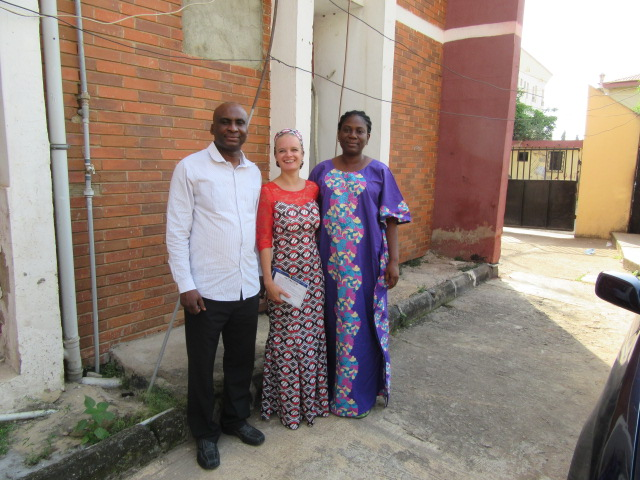
\includegraphics[width=\linewidth]{Chapter_6/conclusion-figure2.JPG}
\caption{Host of My First Field Trip} \label{fig:a}
\end{subfigure}\hspace*{\fill}
\begin{subfigure}{0.485\textwidth}
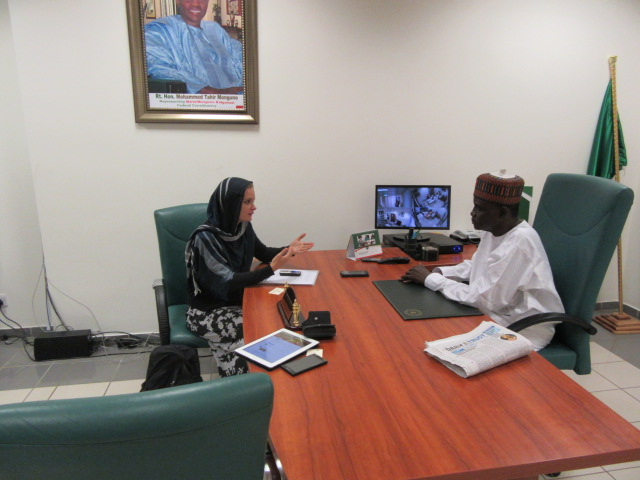
\includegraphics[width=\linewidth]{Chapter_6/conclusion-figure6.JPG}
\caption{In-Depth Interview at the Parliament} \label{fig:b}
\end{subfigure}

\bigskip
\begin{subfigure}{0.485\textwidth}
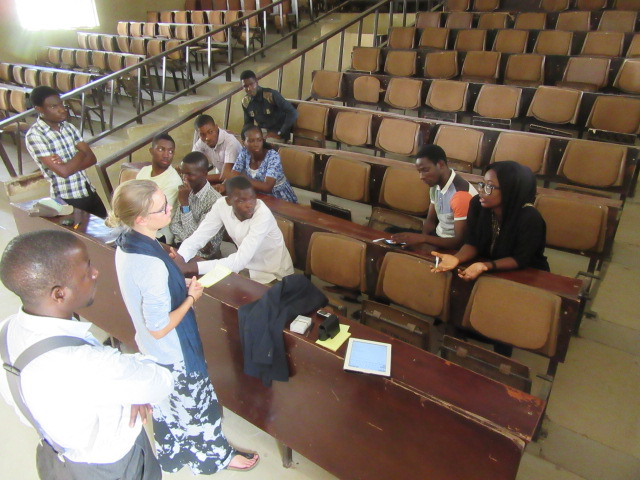
\includegraphics[width=\linewidth]{Chapter_6/conclusion-figure9.JPG}
\caption{FGD with Christian Students} \label{fig:e}
\end{subfigure}\hspace*{\fill}
\begin{subfigure}{0.485\textwidth}
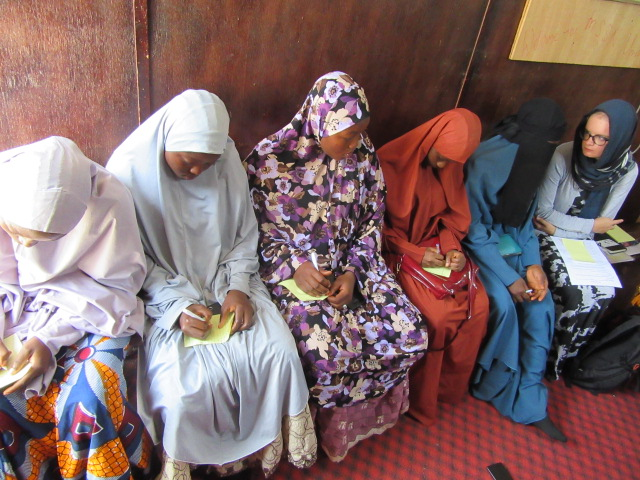
\includegraphics[width=\linewidth]{Chapter_6/conclusion-figure7.JPG}
\caption{FGD with Muslim Students} \label{fig:f}
\end{subfigure}

\bigskip
\begin{subfigure}{0.485\textwidth}
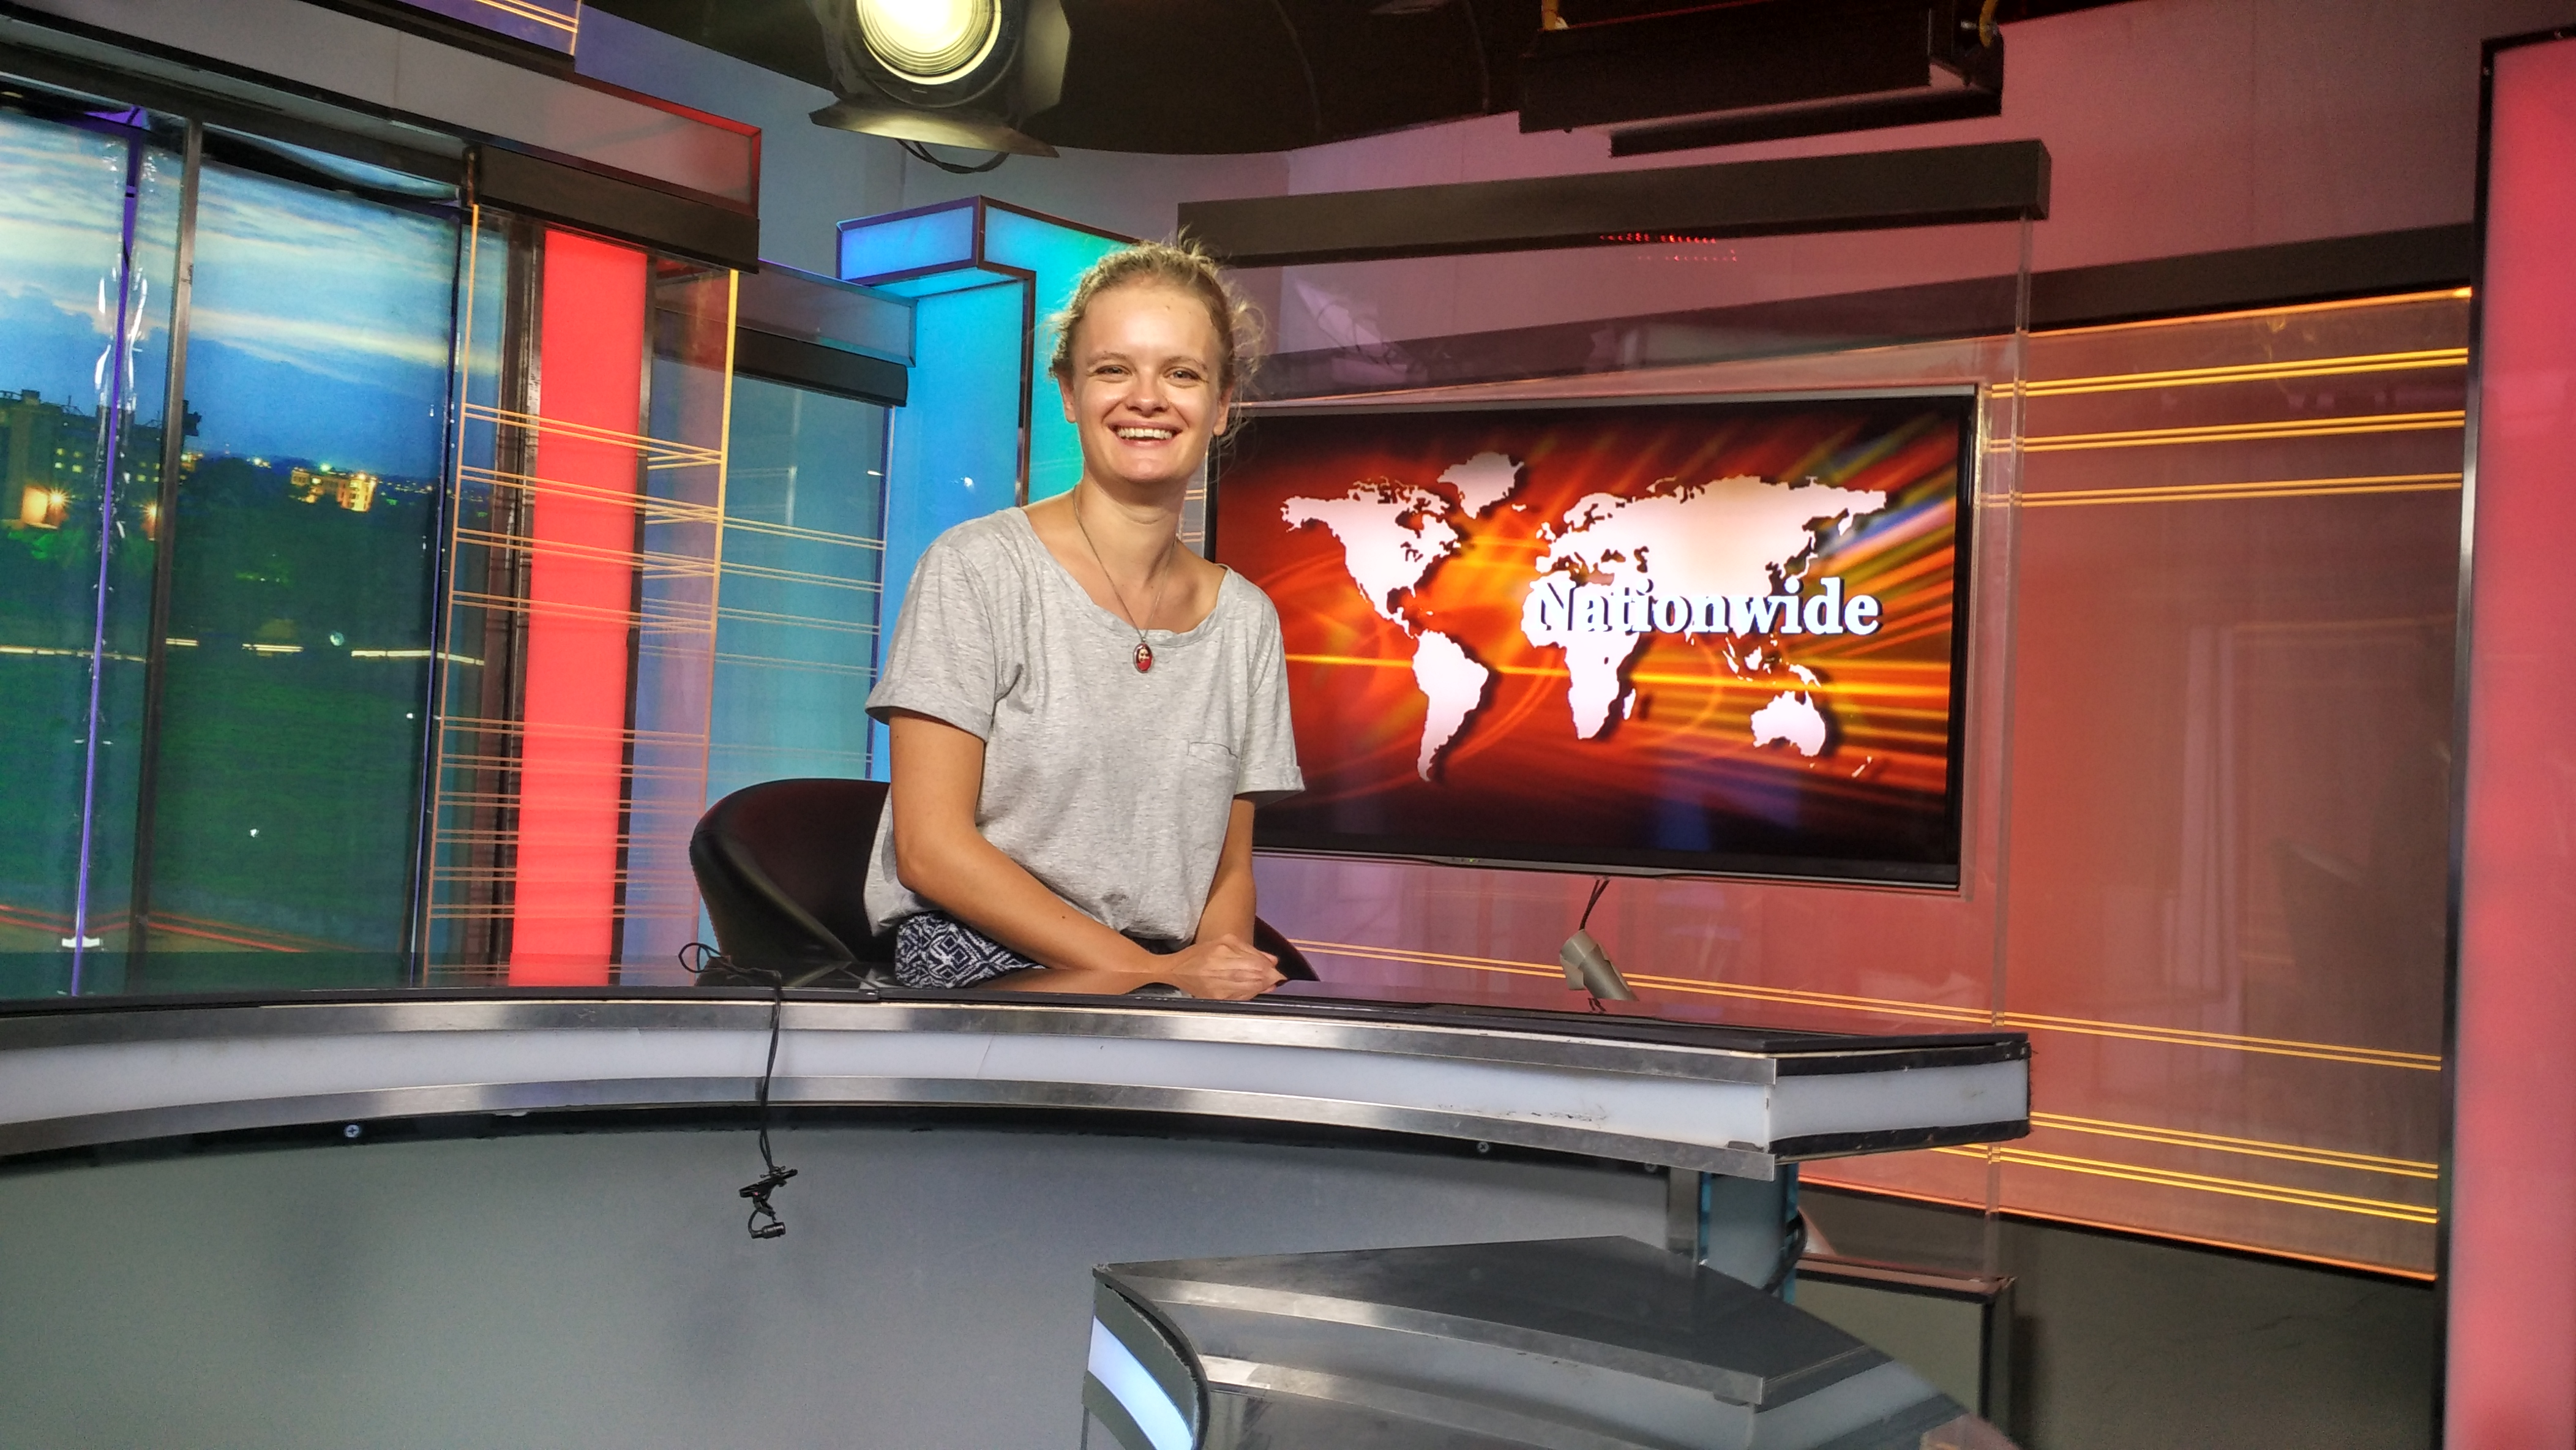
\includegraphics[width=\linewidth]{Chapter_6/conclusion-figure5.jpg}
\caption{After an Interview at a Television Station} \label{fig:c}
\end{subfigure}\hspace*{\fill}
\begin{subfigure}{0.485\textwidth}
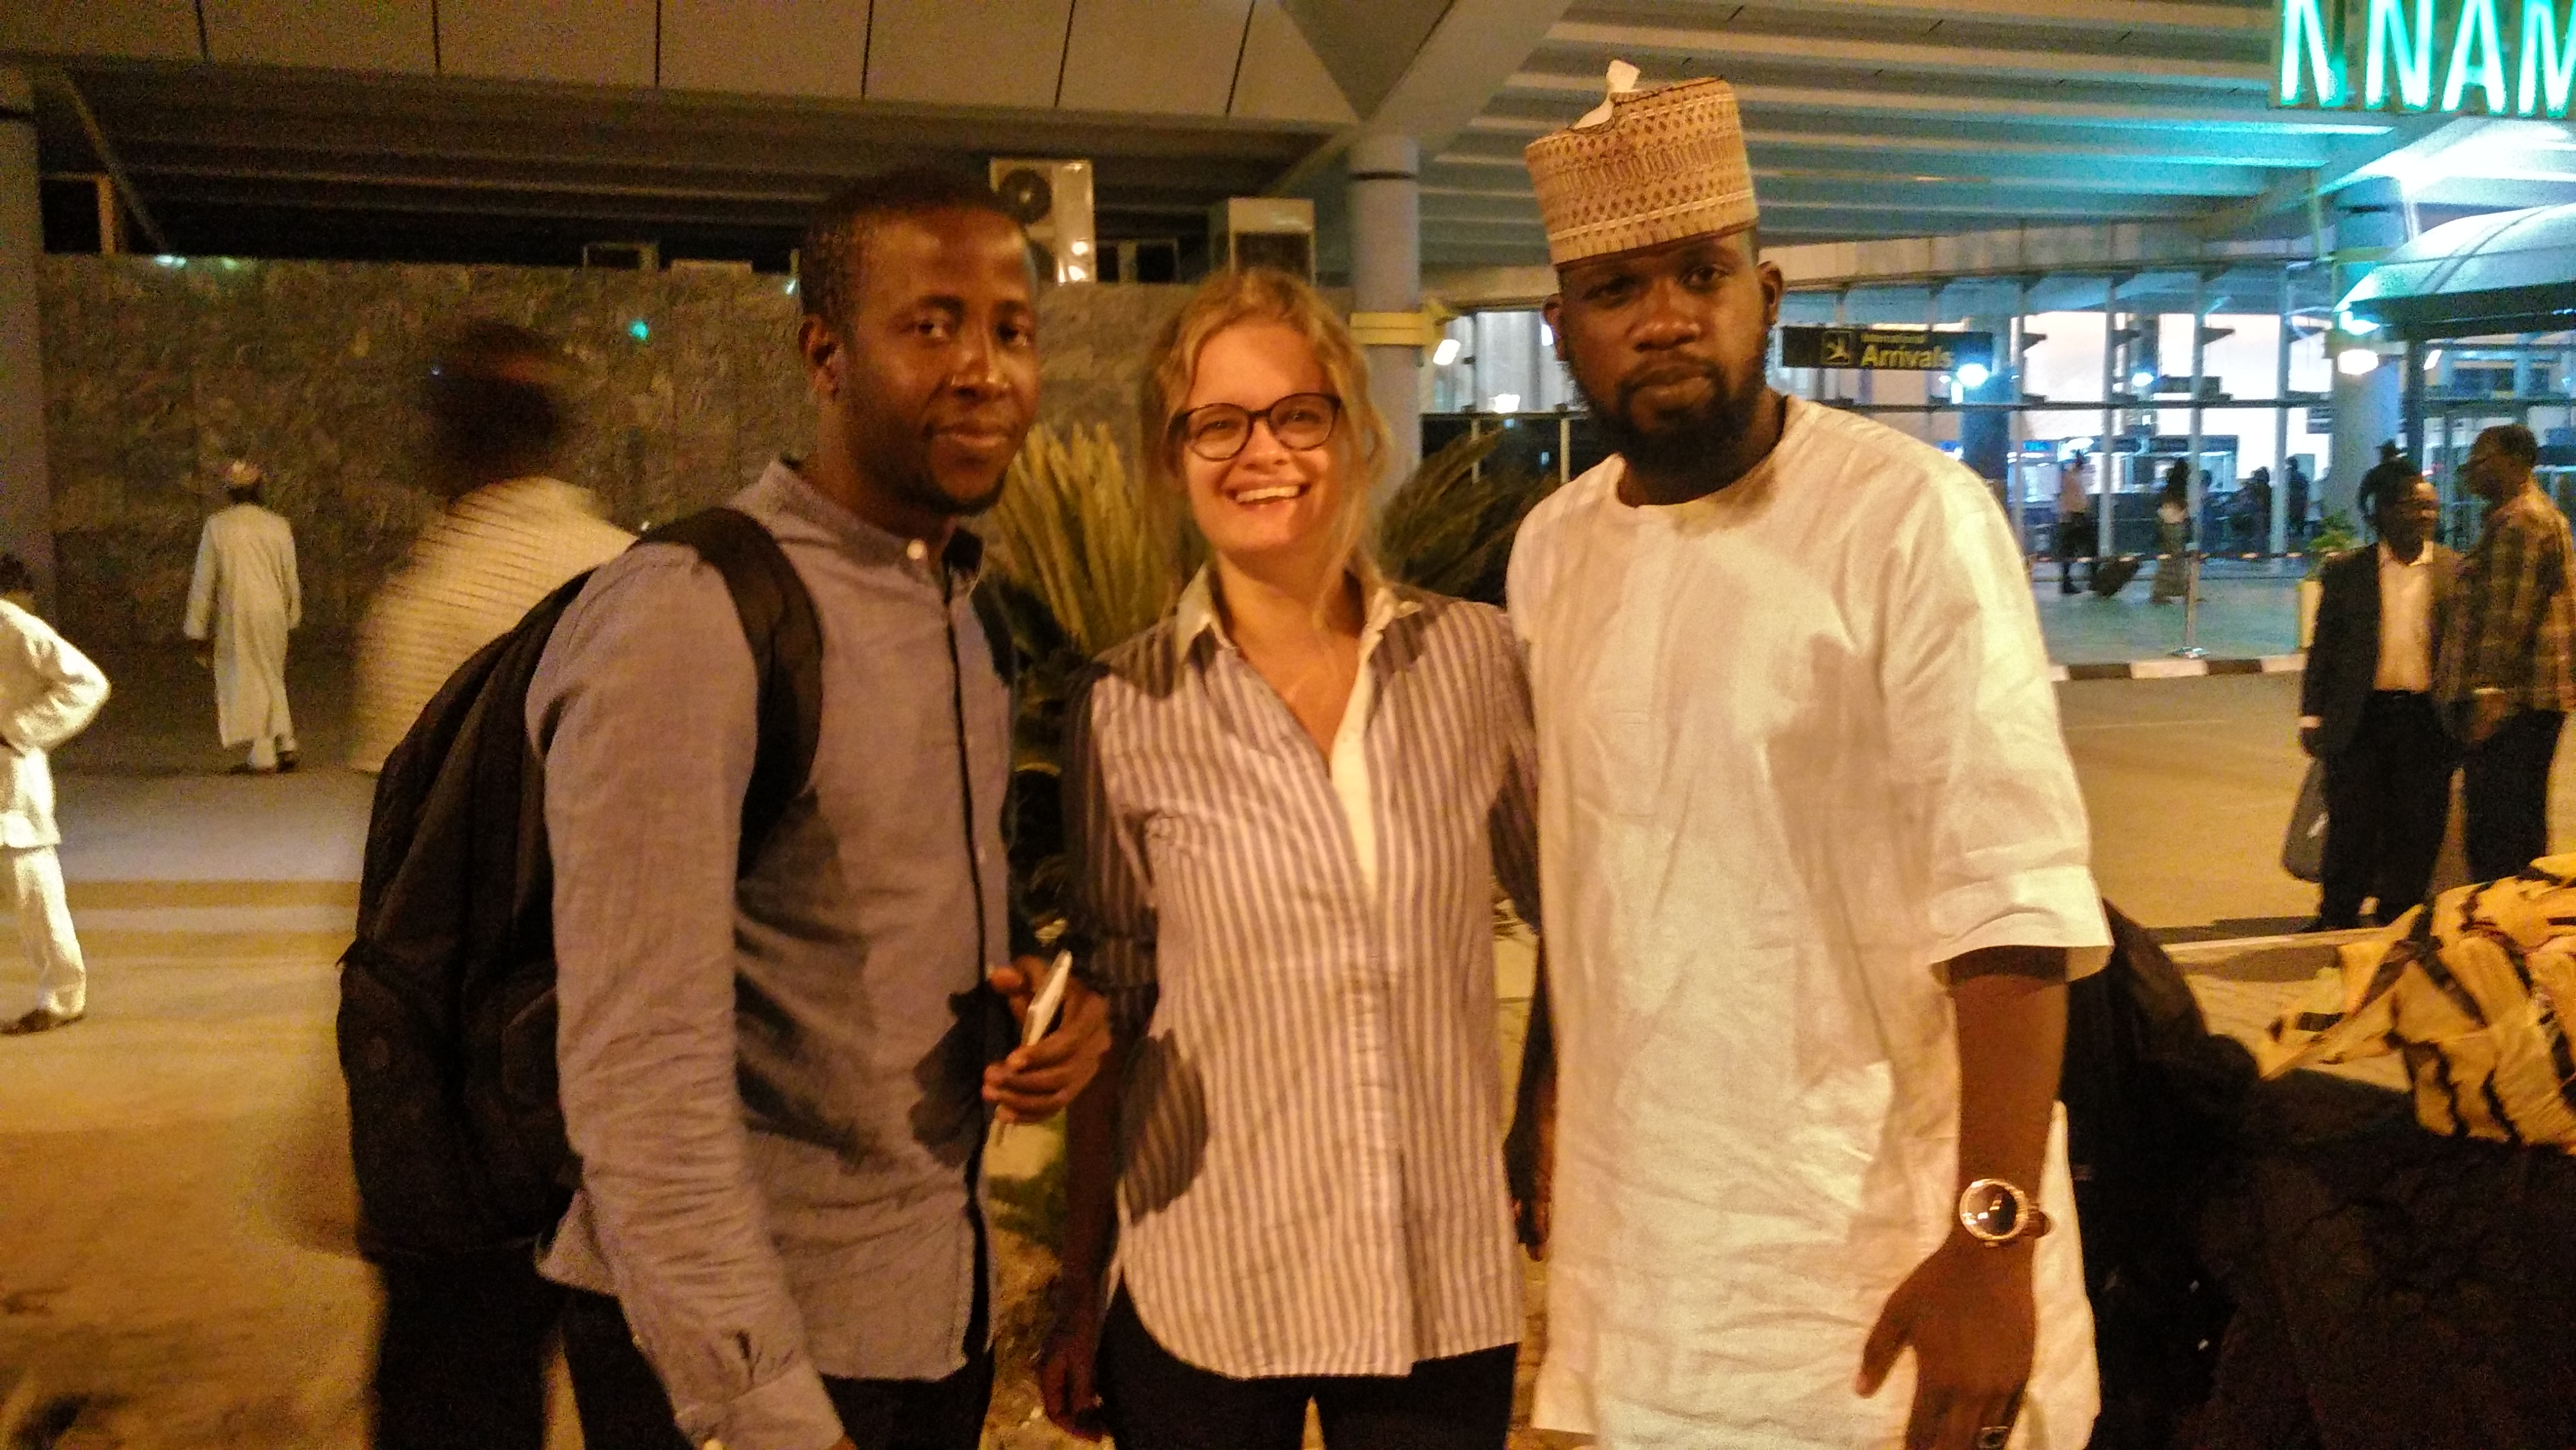
\includegraphics[width=\linewidth]{Chapter_6/conclusion-figure4.jpg}
\caption{My Fieldwork Team} \label{fig:d}
\end{subfigure}

\caption{A Glimpse of My Fieldwork in Nigeria} \label{fig:1}
\end{figure}

\newpage
\subsection{Limitations}
\label{sec:621}
All studies have limitations. Although I tried to answer my research questions as thoroughly as possible, this dissertation also leaves some unanswered and raises further questions. While each empirical chapter was characterized by specific limitations (e.g., the use of cross-sectional data in Chapter 2, a student sample in Chapter 3, idiosyncrasies of the Nigerian case in Chapter 3 and 4, or publication bias in Chapter 5), I now outline how the overall generalizability of this dissertation is also subject to certain limitations.

The first limitation of this dissertation is that \textbf{it did not take time into account}. In fact, this is a twofold limitation. On the one hand, valid concerns can be raised about the generalizability of my results \textit{over time}. Although the duration of the effects was briefly touched upon in Chapter 5, this was not addressed in-depth because this dissertation did not include a panel/longitudinal component. Sniderman and colleagues (\citeyear{Sniderman2019a}) have recently argued in this respect that ``mass reactions to terrorist attacks are limited in size and duration and their end states marked by a return to baselines values of tolerance'' (p. 245). Their heuristic model of public reactions to terrorism is in line with a handful of studies showing that the effects of terrorism on attitudes are often ``short-lived and dissipate rapidly'' \citep[p.~231; see also Dinesen et al., \citeyear{Dinesen2013a}; Economou \& Kollias, \citeyear{Economou2019}]{Arvanitidis2016}. Nevertheless, it is important to note that, although attitudinal responses to terrorism may not be long-lasting, they hold the potential to instigate enduring policies \citep[such as the PATRIOT ACT; see also][]{Tomz2019} and feed the narratives of terrorists \citep{Bail2018}. Therefore, this topic remains worth investigating and longitudinal research designs would be of great added value to this research field---especially given the fact that Chapter 5 clearly showed that public reactions to terrorism are barely studied from a longitudinal perspective. 


On the other hand, much of the studies in my meta-analysis as well as our Nigerian survey offered a one-shot picture at a \textit{peculiar moment in time}---that is, in the post-9/11 era at a time when terrorism was very salient. Hence, one may rightly wonder whether the dynamics of the `idea of terrorism' will play out differently in the future or at times when terrorism is less salient. If another \textit{relevant outgroup} were to commit an act of violence of the same order of magnitude as 9/11, my intergroup framework indeed predicts that the dynamics may change and shift towards that out-group. Next, given the salience of terrorism, as we saw in Chapter 2, the relationship between worrying about terrorism and generalized trust disappeared in those countries where terrorism is almost part of people's daily routine. We also saw that much of our hypotheses were not confirmed in Nigeria---a country characterized by sustained violence. While I have argued that this is to a large extent due to different constellations of the intergroup context, another possibility is that a habituation effect kicks in after a prolonged period of violence. In addition to various empirical findings in this dissertation, several studies conducted in Israel---also a context characterized by protracted conflict/terrorism---tend to support my argument rather than the habituation argument. Scholars have repeatedly documented how exposure to terrorism in Israel is related to increases in exclusionist attitudes toward out-group members \citep{Canetti2009, Canetti-Nisim2009b, Hall2009}, a desire for retaliatory action \citep{Kalagy2017}, and greater authoritarian beliefs and ethnocentrism \citep{Hobfoll2006a}---a relationship often mediated via chronic psychological distress \citep{Canetti-Nisim2009b, Hobfoll2006a}. Importantly, as my meta-analysis showed, these studies predominantly examine attitudes among Israeli Jews toward Palestinians. Hence, again, attitudes towards a stigmatized Muslim minority group are examined among a numerically and politically superior in-group within a context characterized by deep-seated intergroup power hierarchies. 


Second, this dissertation predominantly focused on \textbf{one conceptualization of in- and out-group membership---that is in- and out-groups based on \textit{religion}}. Again, this is a twofold limitation. On the one hand, it entails that much of this dissertation equally examined \textit{Islamist terrorism} and, thereby, falls into the same trap identified in Chapter 5. Of course, I am not detached myself from the intergroup processes central to the main argument of this dissertation. Nevertheless, the main focus on Islamist terrorism in this dissertation was even more the result of using the Global Terrorism Database (Chapter 2), selecting the Boko Haram conflict as an instructive case-study to draw on (Chapter 3 and 4), and inherent biases in this field of study (Chapter 5). On the other hand, I also focused on just \textit{one specific constellation of religious in- and out-groups}. More specifically, I started from the premise that much of today's research on public reactions to terrorism is built on the `white majority'-versus-'Muslim minority' distinction (see also Chapter 5 for a confirmation of this premise). As a result, I deliberately studied Islamist violence within a country where Muslims and Christians constitute about half of the population and representatives from both religious groups hold powerful political positions (i.e., Nigeria). %It is worth noting in this respect that Chapter 2 revealed that concerns over (unspecified) terrorism were related to \textit{increases} in generalized trust in Iraq and Thailand---a Muslim- and Buddhist-majority country, respectively. These are puzzling results worth further scrutiny. 
In short, it remains unclear how violence based on other fault lines affects attitudes within particular societies or how Islamist violence affects attitudes in countries with yet another religious make-up, in particular Muslim-majority countries. These remaining questions bring us to the penultimate section of this dissertation on other promising avenues for future research.


\newpage
\section{Looking Forward: Avenues for Future Research}
\label{sec:63}
Obviously, the list of promising avenues for future research is quasi-endless and includes many of the `usual suspects'---from using more longitudinal research designs to including more representative non-Western samples. Yet, in what follows, I outline four more concrete ideas for future research I am particularly passionate about. These ideas pertain to the four elements central to this dissertation---that is, further work is needed to fully understand the (1) differential labeling of acts/threats of political violence, (2) implications of the intergroup context, (3) complexities of cognitive and affective mediators, and (4) peculiarities of the '4Ps' of public reactions to terrorism.


\subsubsection{Towards a Better Understanding of Labels}
For `terrorism' to change our attitudes, it first needs to be perceived as such. It is surprising in this respect that, so far, very little research has been conducted on the factors that make people classify violent incidents as terrorism \citep[but for an important exception, see][]{Huff2018} and, hence, make particular violent incidents more emotionally and politically powerful. The intergroup perspective at heart of this dissertation holds the potential to explain much of the differential labelling of acts of violence. For example, it might explain why many American politicians, journalists, and citizens tend to react differently to white supremacist terrorism\footnote{Illustratively, in December of 2015, Syed Rizwan Farook and Tashfeen Malik murdered 14 people in San Bernardino, California. The media quickly labelled the attack ‘terrorist,’ the FBI opened a terrorism investigation, and several politicians called for a so-called ‘Muslim ban’ ending immigration from certain Middle Eastern countries in response. Only a few months earlier, in June 2015, Dylann Roof, a White supremacist, murdered nine African American churchgoers in South Carolina. Following this shooting, the media predominantly focused on Roof’s mental health, people fiercely debated whether Roof was as a terrorist or a mass shooter, and he was ultimately charged with nine counts of murder rather than on terrorism grounds \citep{Butler2015}. A handful of studies has also experimentally documented such biases among the general public \citep[e.g.,][]{Piazza2015}.}---violence perpetrated by members of the majority in-group in power---or why Western scholars study these acts of violence differently. Intergroup mechanisms might also explain why communists were often labelled as terrorists in the West throughout the 1960s-1980s---a time with the Soviet Union was seen and treated as an imminent `out-group' threat \citep{Stampnitzky2013}. This thesis aims to encourage future research to deductively test such labeling hypotheses. Particularly, to further contribute to the important question of how terrorism is changing us, it is necessary to causally identify and compare citizens’ differential labeling of a wider range of violent incidents within a more diverse set of countries. Several other features besides intergroup dynamics might be driving these responses but, to date, no research has carefully disentangled the effect of those factors. For example, how does past micro- and macro-level exposure to political violence affect how information concerning a new threat is processed? For example, will Norwegians be more inclined to label acts of extreme-right violence `terrorist' as a result of the Ut{\"{o}}ya attacks? Or, how does information about a new threat, coming from particular media outlets and/or political elites, interact with intergroup dynamics to affect how we label, perceive, and react to threats?



\subsubsection{Towards a Broader Understanding of Intergroup Contexts}
More broadly, research is needed to replicate the findings of this dissertation and to explore the generalizability of its main conclusion regarding the importance of the intergroup context. In other words, this avenue for future research is more extensive than understanding differential labeling; it is about getting a better understanding of both labels and responses across a wider range of intergroup contexts. For example, government officials in Beijing have recently proposed a new security law, radically changing Hong Kong's unique status, as ``terrorism is growing in the city'' (BBC News, 2020). China's intergroup context is not so much characterized by the `White majority'-`Muslim minority' divide,\footnote{Yet, see also its recent repression of the Uyghurs---a predominantly Muslim ethnic minority in Northwest China \citep{Chestnut2020}.} but rather by geographic-political identities. Another constellation of social identities might also be one's political identity. Intergroup dynamics might help us to explain why Donald Trump---a Republican President---recently urged to designate ANTIFA---a left-wing activist movement---as a `terrorist organization' \citep{Trump2020}, but also why left-wing academics, journalists, and politicians repeatedly urge society to designate and treat white supremacists as `terrorists' \citep{Meier2020b}. If the debate on public reactions to terrorism is to be moved forward, a better understanding of the implications of such different constellations of social identities needs to be developed. This dissertation provides one of the first attempts to explore and theorize about the implications of the intergroup context in which violence takes place, and future studies could build on this work by developing and testing (e.g., using qualitative comparative analysis techniques) a classification scheme that predicts which intergroup identities may lead to which labeling and attitudinal differences in which specific societies. Such in-depth and nuanced information on the repercussions of different conceptualizations of social identities would help us to establish a greater degree of accuracy on this matter.


\subsubsection{Towards a Person-Centered Understanding of Mediators}
Third, as said before, a central feature within political psychology is the role of concrete cognitions and emotions in driving public reactions to terrorism. Perceptions of threat and insecurity, often linked to the emotion of fear, are thought to affect sociopolitical attitudes in a different way compared to perceptions of moral violations and injustice, often linked to the emotion of anger. To assess these hypotheses, almost all previous studies rely on a variable-centered approach using factor analysis to measure discrete cognitions and emotions. Yet, a person-centered approach using latent class analysis (LCA) could complement this variable-centered approach and generate new insights on the role of cognitions and emotions. More specifically, instead of examining the impact of one or more cognitions and/or emotions, one could study how \textit{distinct groups of individuals}, characterized by particular combinations of cognitions and emotions, react differently to terrorism. In other words, LCA allows us to model a greater deal of heterogeneity in how citizens react to violence by identifying subgroups or classes of individuals who share similar patterns of affective and/or cognitive responses to terrorism---which might be more in line with what happens in reality. For example, some people might be outraged and anxious at the same time, others might be just angry, and yet others might be afraid without holding a moral grudge. After identifying such subgroups, one can examine whether they develop different sociopolitical attitudes. In short, extending the dominant factor analytic framework using latent class models would be worthwhile.


\subsubsection{Towards a Less Biased Understanding of Outcomes}
Last, until now, public reactions to terrorism have mainly been studied from the perspective of the dominant majority group and the studied attitudes often relate to a stigmatized minority group (e.g., anti-immigration attitudes, prejudice against Muslims/Arabs, etc.). A greater focus on the perspectives of minorities as well as on a wider range of outcome measures could produce interesting findings allowing for more nuance in the literature. In a similar vein, recent work in social psychology has highlighted a liberal bias in the study of prejudice and cautioned that results might be an artifact of a one-sided focus on prejudice towards groups that liberals prioritize \citep{Brandt2014a, Reyna2018}. These ideas might be applicable to the field of terrorism effects studies as well, where scholars tend to focus on outcome measures that are conservative in nature (e.g., support for anti-immigration policies or military actions). How results change when using less skewed outcome measures calls for further scrutiny.



\newpage
\section{One Final Thought}
\label{sec:64}
The story I have told is a story full of concepts, theories, and numbers. As I often realized over the past five years, it can be hard at times to look through the data and see the people behind the numbers. So just remember, every number you have seen told you something about angry and anxious citizens, about people who discriminate and are discriminated against, or about young and strong Nigerians trying to cope with an extremely violent insurgency. As a result, the story I have told is also a predominantly negative one. It is a story about losses and destruction, anger and anxiety. Yet, despite this bleak picture, I want to end this dissertation a more positive note because \dots

\vspace{0.5cm}

\epigraph{ \dots democracy does require a basic sense of solidarity---the idea that for all our outward differences, we're all in this together; that we rise or fall as one.}{\textit{Barack Obama \\ Farewell Address, January 10, 2017}}

So, let us try to \dots

\epigraph{ \dots don't be afraid. Be focused. Be determined. Be hopeful. Be empowered. [...]. Lead by example with hope, never fear.}{\textit{Michelle Obama \\ Final Address, January 6, 2017}}


\clearpage



